\chapter{Introduzione al lavoro}\label{ch:capitolo2}

\section{Blender}\label{ch:2.1}
Mininet è uno strumento di simulazione di reti che permette di creare topologie grandi e complesse e che supporta reti di tipo SDN basate sul protocollo OpenFlow.\\\\
Le idee chiave su cui è basato Mininet sono:
\begin{itemize}
	\item \textit{Flessibilità}: nuove topologie e funzioni sono implementate via software, usando linguaggi di programmazione diffusi e sistemi operativi comuni
	\item \textit{Applicabilità}: le implementazioni su reti simulate devono poter funzionare anche su reti reali
	\item \textit{Interattività}: la gestione ed il funzionamento delle reti simulate devono essre in tempo reale, come avverebbe in una rete vera
	\item \textit{Scalabilità}: l'ambiente di prototipazione deve essere in grado di simulare grandi quantità di host e switch su un solo computer
	\item \textit{Realismo}: il comportamento della rete simulata deve rispecchiare con un buon livello di confidenza quello della rete reale, in modo da poter implementare applicazioni e protocolli senza modifiche al codice
	\item \textit{Condivisibilità}: i prototipi creati devono essere facilmente condivisibili con altri collaboratori che a loro volta possano eseguire e modificare le simulazioni \cite{mn2}
\end{itemize}

\subsection{Installazione}\label{ch:2.1.1}
Il modo più semplice per utilizzare Mininet è scaricare dal sito ufficiale una versione modificata di Ubuntu 14.04 nella quale sono preinstallati, oltre a Mininet, OpenFlow e vari programmi utili per la gestione e l'analisi delle reti.\\
Questo Sistema Operativo può poi essere installato su una macchina virtuale. All'accensione si presenta privo di un'interfaccia grafica, che è tuttavia possibile installare. Per utilizzarlo è quindi opportuno conoscere i comandi fondamentali per utilizzare Linux da linea di comando.\\\\
Dopo l'installazione, l'accensione ed il login, l'interfaccia che si presenta all'utilizzatore è questa:
\begin{figure}[h!]
	\centering
	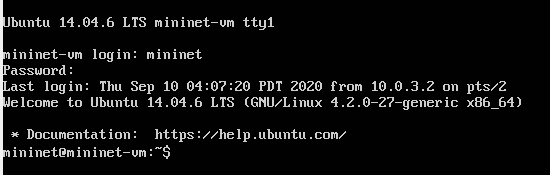
\includegraphics[width=1\linewidth]{../immagini/mn}
	\caption[Interfaccia di Mininet]{Interfaccia a linea di comando di Mininet all'accensione}
	\label{fig:mn}
\end{figure}
\subsection{Avvio di Mininet}\label{ch:2.1.2}
Pr avviare Mininet è necessario usare il comando "mn" con i permessi di root, quindi "sudo mn".\\
In questo modo si crea la topologia di default, composta da due host, uno switch ed un controller. È anche possibile creare topologie personalizzate tramite uno script Python da eseguire all'avvio.\\
Ci si trova quindi davanti la \textit{CLI (Command Line Interface)} di Mininet. Ciascun host possiede a sua volta una CLI in grado di eseguire tutti i comandi di una normale macchina Linux. Per farlo è sufficiente scrivere il nome dell'host sul quale si vuole eseguire il comando, seguito dal comando stesso.
\subsection{Gestione della rete}\label{ch:2.1.3}
Mininet mette a disposizione dei comandi specifici per poter monitorare lo stato della rete. Il seguente elenco spiega alcuni tra i comandi principali e la loro applicazione alla topologia di default.
\begin{itemize}
	\item \textit{mininet> nodes}\\
	Questo comando genera un elenco di tutti i nodi. Nel caso in esame i nodi sono h1, h2, s1 e c0.
	\item \textit{mininet> net}\\
	Si usa questo comando per conoscere le interfacce tramite cui sono collegati i nodi. In questo caso l'interfaccia eth0 dell'host h1 è collegata all'interfaccia eth1 dello switch s1, mentre l'interfaccia eth0 dell'host h2 è collegata all'interfaccia eth2 dello switch s1.
	\item \textit{mininet> dump}\\
	Questo comando mostra gli indirizzi IP e gli ID dei processi dei singoli nodi. Possiamo notare che l'indirizzo IP di h1 è 10.0.0.1 con ID del processo uguale a 6806, mentre l'indirizzo di h2 è 10.0.0.2 con Id del processo uguale a 6808.
	\item \textit{mininet> link s1 h1 down/up}\\
	Questi comandi vengono usati per disattivare o attivare una connessione. È possibile vedere l'effetto di questa azione provando ad eseguire tra i due nodi interessati un ping che, se la connessione non è attiva, fallirà.
	\item\textit{mininet> h1 ping s1}\\
	Si usa questa sintassi per effettuare un ping. In particolare, si utilizza il comando "ping", utilizzabile normalmente su linux, specificando il nodo che deve eseguire l'azione, h1, e il nodo destinazione, s1. Per \textit{pingare} tutti i nodi si usa il comando \textit{"pingall"}.
	\item\textit{mininet> h1 ifconfig -a}\\
	Anche questo comando è presente di base in tutte le macchine linux. Utilizzato in questo modo serve per visualizzare tutte le informazioni, tra cui indirizzo IP, MAC e netmask, sulle connessioni di h1.
\end{itemize}
\begin{figure} [h!]
	\centering
	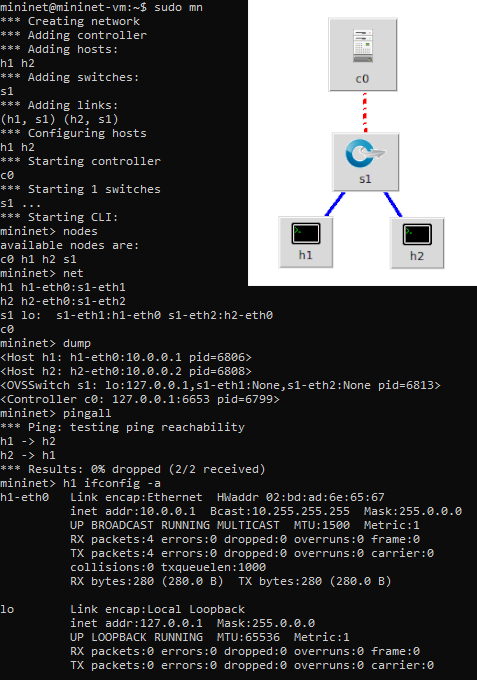
\includegraphics[width=0.97\linewidth]{../immagini/mn/4b}
	\caption[Comandi di base su Mininet]{Utilizzo dei comandi di base di Mininet applicati alla topologia di default, rappresentata in alto a destra.}
	\label{fig:4b}
\end{figure}
\subsection{Topologie complesse}\label{ch:2.1.4}
È ovviamente possibile creare topologie più elaborate rispetto a quella di default.\\
Per farlo bisogna specificare il parametro \textit{"--topo"} quando si esegue \textit{"sudo mn"}.\\
Ad esempio, con il comando
\begin{center}
	\textbf{sudo mn --topo linear,3}
\end{center}
si crea una topologia composta da 3 host, ciascuno connesso ad uno switch. Se invece eseguiamo il comando
\begin{center}
	\textbf{sudo mn --topo single,3}
\end{center}
creiamo una topologia composta da 3 host, tutti connessi allo stesso switch.\\\\
È tuttavia possibile personalizzare ulteriormente le topologie da simulare. Per farlo si possono utilizzare le API Python di Mininet\\
\begin{lstlisting}[language=Python]
from mininet.topo import Topo

class MyTopo( Topo ):
	"Simple topology example."

	def __init__( self ):
		"Create custom topo."

		# Initialize topology
		Topo.__init__( self )

		# Add hosts and switches
		h1 = self.addHost( 'h1' )
		h2 = self.addHost( 'h2' )
		h3 = self.addHost( 'h3' )
		h4 = self.addHost( 'h4' )
		s1 = self.addSwitch( 's1' )
		s2 = self.addSwitch( 's2' )

		# Add links
		self.addLink( h1, s1 )
		self.addLink( h2, s1 )
		self.addLink( s1, s2 )
		self.addLink( s2, h3 )
		self.addLink( s2, h4 )

topos = { 'mytopo': ( lambda: MyTopo() ) }
\end{lstlisting}
La prima riga serve per importare le API di Mininet. L'elenco completo si trova sul sito \textit{http://mininet.org/api}.\\
Possiamo identificare i comandi principali del codice:
\begin{itemize}
	\item \textit{addHost} aggiunge un host alla topologia e fornisce in uscita il nome
	\item \textit{addSwitch} aggiunge uno switch alla topologia e fornisce in uscita il nome
	\item \textit{addLink} aggiunge una connessione bidirezionale tra i due nodi specificati
\end{itemize}
È quindi evidente che la topologia così creata sia composta da 4 host (h1, h2, h3 e h4) divisi in due coppie, ciascuna delle quali è connessa ad uno switch (s1 e s2), a loro volta connessi.\\
Questo codice può essere eseguito tramite il comando
\begin{center}
	\textbf{sudo mn --custom esempio.py --topo mytopo}
\end{center}
dove il parametro \textit{--custom} serve per specificare il percorso e il nome del file python, mentre \textit{--topo} permette di scegliere il nome della topologia da usare.\\\\
Durante la fase di creazione della topologia è possibile specificare anche altri parametri. Ad esempio, con il comando
\begin{center}
	\textbf{self.addLink(host, switch,
bw=10, delay='5ms', loss=10)}
\end{center}
si crea un link con banda pari a 10Mbps, ritardo di 5ms, 10\% di probabilità d'errore.\\
 Altri esempi verranno forniti nel prossimo capitolo, dove verrà costruita una topologia per la quale sarà necessario utilizzare queste funzioni. \cite{mn3}

\section{OpenFlow}\label{ch:2.2}
OpenFlow è il primo protocollo standardizzato per le reti SDN. Lo scopo del protocollo è di permettere l'accesso al piano di controllo di un router o di uno switch tramite la rete.\\\\
L'idea di base è quella di dividere il traffico in \textit{flussi}. Un flusso è un insieme di pacchetti contraddisitinti da caratteristiche comuni, come ad esempio la porta TCP o l'indirizzo IP o MAC di partenza.\\
Questi flussi sono organizzati in \textit{flow tables}, ovvero tabelle nella quale viene specificato come il dispositivo possa identificare i pacchetti appartenenti ad un certo flusso e l'azione da eseguire su di essi. \\
Il controller è in grado di accedere a queste tabelle di flusso ed è in grado di modificarne dinamicamente le regole.\\
\begin{figure}[h!]
	\centering
	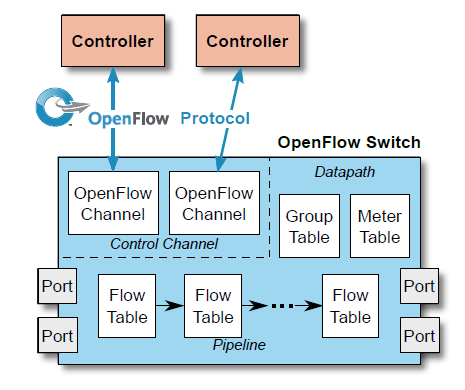
\includegraphics[width=0.85\linewidth]{../immagini/of}
	\caption[Protocollo OpenFlow]{Struttura del protocollo openFlow, che permette di accedere al piano di controllo tramite la rete}
	\label{fig:of}
\end{figure}\\
Il protocollo OpenFlow può essere applicato a router e switch già esistenti, ciascuno dei quali già presenta delle flow tables, senza la necessità di doverli riprogrammare. Si crea quindi uno Switch OpenFlow, caratterizzato dalle tabelle di flusso e dal canale sicuro per poter comunicare con il controller.\\
Switch e controller devono poter comunicare non solo per permettere a quest'ultimo di modificare le tabelle di flusso, ma anche per permettere allo switch di inviare pacchetti al controller stesso nel caso in cui non sappia come comportarsi con essi. \cite{of}\\\\
Mininet è spesso utilizzato per simulare reti di tipo SDN anche grazie al suo supporto di OpenFlow stesso. In fase di creazione di una topologia, infatti, è possibile specificare la tipologia degli switch.\\
Gli switch che supportano OpenFlow si chiamano OpenvSwitch (OVS) e posseggono una serie di comandi per la loro gestione e per la creazione ed organizzazione delle flow tables.\\
I principali sono:
\begin{itemize}
	\item \textit{mininet> sh ovs-ofctl show s1}\\
	Fornisce informazioni sullo switch s1, tra cui dati su porte e flow tables
	\item \textit{mininet> sh ovs-ofctl dump-tables s1}\\
	Questo comando mostra un elenco delle tabelle di s1 e le relative informazioni
	\item \textit{mininet> sh ovs-ofctl dump-ports s1}\\
	Questo comando mostra i dispositivi della rete collegati allo switch e i relativi dati.
	\item \textit{mininet> sh ovs-ofctl add-flow s1 flow}\\
	Si usa questo comando per aggiungere un flusso nella flow table di s1. È necessario specificare le caratteristiche che accomunano i pacchetti appartenenti
\end{itemize}
Alcuni di questi comandi verranno messi in pratica nel prossimo capitolo. \cite{ovs}

\section{Strumenti di analisi prestazionale}\label{ch:2.3}
Una caratteristica fondamentale di un programma come Mininet è la possibilità di poter misurare le prestazoni delle reti che si stanno analizzando. Linux ci fornisce diversi strumenti che ci permettono di fare ciò.
\begin{itemize}
	\item \textbf{Ping}\\
	Questo è senza dubbio lo strumento più semplice che abbiamo a disposizione per testare la comunicazione tra due dispositivi. Viene solitamente usato per verificare il funzionamento e la latenza nella connessione tra due dispositivi.\\
	La sintassi del comando è
	\begin{center}
		\textbf{ping \{destinazione\} [opzioni]}
	\end{center}
	Nell'esempio possiamo vedere un esempio di utilizzo del comando \textit{ping} applicato agli host \textit{h1} e \textit{h2} della topologia di default. Il parametro \textit{-c} serve per specificare quanti pacchetti di test inviare.
	\begin{figure}[h!]
		\centering
		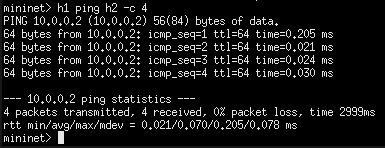
\includegraphics[width=0.85\linewidth]{../immagini/mn/ping}
		\caption[Comando "ping"]{Utilizzo del comando "ping"}
		\label{fig:ping}
	\end{figure}
	 
	\item \textbf{Nmap}\\
	Uno dei limiti del comando \textit{ping} è l'impossibilità di specificare la porta TCP della quale effettuare la verifica. \textit{Nmap} ha un funzionamento molto simile al comando precedente, ma ci mette a disposizione questa funzione. Questa possibilità ci sarà molto utile quando, nel prossimo capitolo, avremo bisogno di verificare la latenza della rete per i diversi servizi richiesti.\\
	La sintassi del comando è
	\begin{center}
		\textbf{nmap -p [n° porta] \{destinazione\}}
	\end{center}
	Nell'esempio vediamo l'utilizzo di \textit{nmap} tra i due host della topologia di default sulla porta TCP 80.
	\begin{figure}[h!]
		\centering
		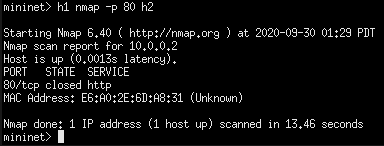
\includegraphics[width=0.85\linewidth]{../immagini/mn/nmap}
		\caption[Comando "nmap"]{Utilizzo del comando "nmap"}
		\label{fig:nmap}
	\end{figure}
	\item \textbf{Iperf}\\
	La latenza non è l'unico parametro che è possibile misurare.\\È infatti possibile monitorare anche la banda dei collegamenti, tramite il comando \textit{iperf}.\\Per utilizzarlo è necessario impostare uno dei due host come server e uno come client. Non è quindi possibile utilizzare direttamente il comando, è prima necessario aprire un terminale separato per ciascun host scrivendo nella CLI di Mininet
	\begin{center}
		\textbf{mininet> xterm h1 h2}
	\end{center}
	Bisogna poi utilizzare \textit{iperf} per impostare uno dei due host come server e l'altro come client.\\
	La sintassi del comando per il server è
	\begin{center}
		\textbf{iperf -s -p [n° porta]}
	\end{center}
	La sintassi del comando per il client è
	\begin{center}
		\textbf{iperf -c \{destinazione\} -p [n° porta]}
	\end{center}
	Nell'esempio h2 è il server e h1 è il client e i due comunicano sulla porta TCP 80.
	\begin{figure}[h!]
		\centering
		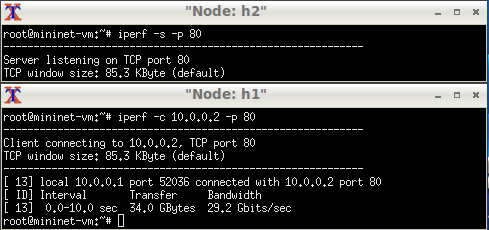
\includegraphics[width=0.85\linewidth]{../immagini/mn/iperf}
		\caption[Comando "iperf"]{Utilizzo del comando "iperf"}
		\label{fig:iperf}
	\end{figure}
	\item \textbf{Wireshark}\\
	A differenza dei precedenti comandi, Wireshark è un vero e proprio programma dotato di interfaccia grafica. Il suo scopo è quello di "catturare" il traffico lungo una connessione, per poter analizzare i pacchetti che vengono inviati durante una trasmissione di dati.\\
	Per avviarlo è sufficiente utilizzare da terminale il comando
	\begin{center}
		\textbf{sudo wireshark}
	\end{center}
	dopo essersi assicurati di avere a disposizione un'interfaccia grafica.\\
	Nella figura 2.7 possiamo vedere come appare il programma all'apertura. Se, dopo aver selezionato l'interfaccia \textit{s1-eth1}, che nella topologia di default di Mininet corrisponde all'interfaccia di s1 collegata ad h1, avviamo un ping sulla porta TCP 80 tramite il comando \textit{nmap} mostrato nell'esempio in figura 2.5, osserviamo il traffico catturato nell'immagine 2.8. Possiamo notare che i pacchetti sono di tipo \textit{http}, che è appunto il servizio associato alla porta TCP 80. \cite{ws}\\
	\begin{figure}[h!]
		\centering
		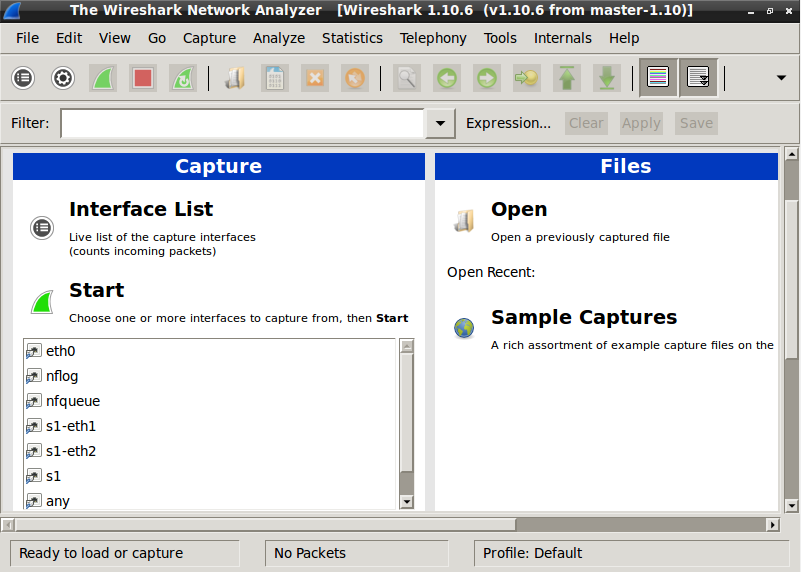
\includegraphics[width=0.9\linewidth]{../immagini/mn/wireshark1}
		\caption[Interfaccia di Wireshark]{Interfaccia grafica di Wireshark all'accensione}
		\label{fig:wireshark1}
	\end{figure}
	\begin{figure}[h!]
		\centering
		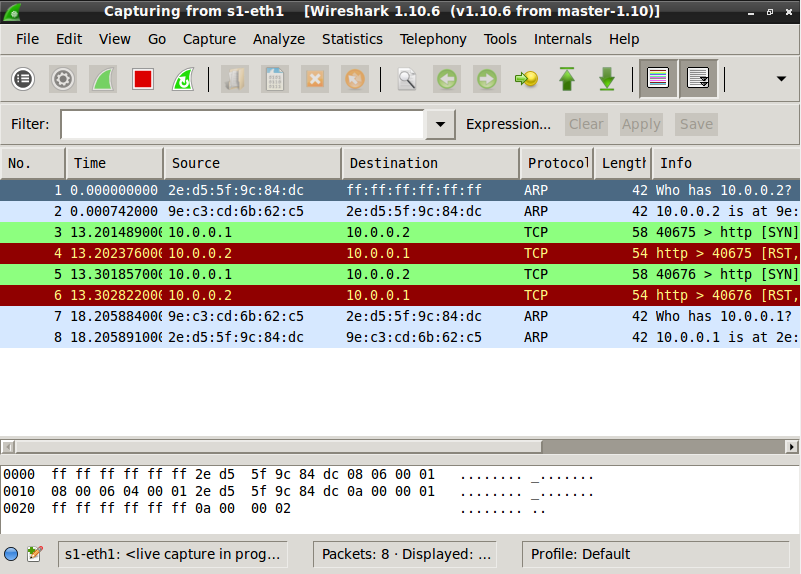
\includegraphics[width=0.9\linewidth]{../immagini/mn/wireshark}
		\caption[Utilizzo di Wireshark]{Esempio di utilizzo di Wireshark per la cattura di pacchetti}
		\label{fig:wireshark}
	\end{figure}
\end{itemize}
Ovviamente questi sono solo alcuni degli innumerevoli strumenti che Mininet e l'ambiente Linux in generale mettono a disposizione.\\
I comandi ed i programmi spiegati in questo capitolo verranno messi in pratica nel prossimo capitolo per la simulazione di una rete basata sul concetto di Network Slicing.\\
La topologia della rete verrà costruita con i comandi mostrati. Verranno poi analizzate le prestazioni per vari servizi prima e dopo averla programmata grazie al protocollo OpenFlow e verranno infine confrontate.